\chapter{INFRASTRUCTURE SBT \& CERTIFICATION}
\label{chap:sbt_infrastructure}

La certification RBK 2.0 n'est pas un fichier PDF. C'est une preuve cryptographique on-chain, incensurable et composable, matérialisée par un Soulbound Token (SBT).

\section{Philosophie : "Don't Trust, Verify"}

Contrairement aux diplômes traditionnels (facilement falsifiables), le SBT RBK est :
\begin{itemize}
    \item \textbf{Permanent :} Ancré sur la blockchain (Solana/Polygon).
    \item \textbf{Révocable :} En cas de triche avérée post-diplomation (mécanisme de slashing).
    \item \textbf{Riche :} Contient des métadonnées prouvant les compétences (liens vers repos, hash des commits).
\end{itemize}

\section{Stack Technique SBT}

\subsection{Choix du Standard}
Nous utilisons une architecture hybride optimisée pour le coût et la performance.
\begin{itemize}
    \item \textbf{Réseau :} Polygon POS (compatibilité EVM, frais nuls pour l'utilisateur) ou Solana (Compressed NFTs pour le volume).
    \item \textbf{Standard :} ERC-5192 (Minimal Soulbound NFTs) sur EVM.
\end{itemize}

\begin{techBox}{Interface SBT (Solidity)}
\begin{lstlisting}[language=C++]
interface ISoulbound {
    /// @notice Émis quand un SBT est minté. Locké par défaut.
    event Locked(uint256 tokenId);
    /// @notice Le transfert est impossible sauf pour le burn (révocation).
    function locked(uint256 tokenId) external view returns (bool);
    /// @notice Seul l'admin (Smart Contract RBK) peut révoquer.
    function revoke(uint256 tokenId) external onlyRole(ADMIN);
}
\end{lstlisting}
\end{techBox}

\section{Cycle de Vie de la Certification}
\begin{figure}[H]
    \centering
    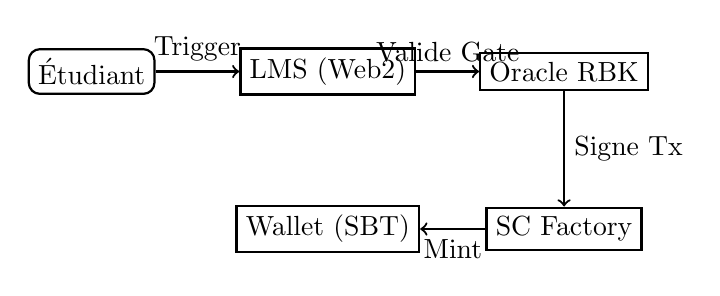
\begin{tikzpicture}[node distance=2cm, auto, thick]
        \node (student) [draw, rectangle, rounded corners] {Étudiant};
        \node (lms) [draw, rectangle, right of=student, node distance=3cm] {LMS (Web2)};
        \node (oracle) [draw, rectangle, right of=lms, node distance=3cm] {Oracle RBK};
        \node (factory) [draw, rectangle, below of=oracle] {SC Factory};
        \node (wallet) [draw, rectangle, left of=factory, node distance=3cm] {Wallet (SBT)};

        \draw[->] (student) -- node {Trigger} (lms);
        \draw[->] (lms) -- node {Valide Gate} (oracle);
        \draw[->] (oracle) -- node {Signe Tx} (factory);
        \draw[->] (factory) -- node {Mint} (wallet);
    \end{tikzpicture}
    \caption{Workflow d'Émission Automatisé}
\end{figure}

\section{Conformité RGPD \& Privacy}

La blockchain est publique, mais les données personnelles ne le sont pas.
\begin{itemize}
    \item \textbf{On-Chain :} Uniquement l'ID étudiant (pseudonyme) et le Hash des compétences.
    \item \textbf{Off-Chain (IPFS/Private) :} Le "Verifiable Credential" complet (Nom, Prénom, Notes détaillées).
    \item \textbf{Droit à l'oubli :} L'étudiant peut demander le "Burn" de son token pour effacer sa trace on-chain.
\end{itemize}

\section{Cas d'Usage : Le Recrutement Instantané}

Les partenaires B2B (Job Board) peuvent interroger le Smart Contract pour filtrer les candidats : "Montre-moi tous les wallets qui détiennent le SBT 'Solana Advanced' ET le SBT 'Security Auditor'." Cela réduit le temps de screening de plusieurs jours à quelques millisecondes.
